\documentclass[hyperref={unicode=true},professionalfont]{beamer}
% \usetheme{Warsaw}
\usepackage{newtxtext,newtxmath}

% \documentclass[hyperref={unicode=true}]{beamer}

\usepackage[russian]{babel}
 \usepackage[T2A]{fontenc}
\usepackage[utf8]{inputenc}
\usepackage[unicode=true]{hyperref}
% \usepackage{cyrtimes}


\usepackage{amsmath,amssymb,longtable,hhline}
\usepackage{mathrsfs}
\usepackage{multimedia}
\usepackage{tcolorbox}
\usepackage{framed}
\usepackage{setspace}
\usepackage{marvosym}

\usepackage{tabularx}
\usepackage{multirow}
\usepackage{multicol}
\usepackage{array}
\usepackage{adjustbox}

\usepackage[labelsep=period]{caption}
\setbeamertemplate{caption}[numbered]

\usetheme{Boadilla}

% \usepackage{lmodern}

\setbeamertemplate{navigation symbols}{}
 
%Подписи к таблицам и рисункам
\usepackage[tableposition=top,font=large]{caption}
\usepackage{subcaption}
\DeclareCaptionLabelFormat{gostfigure}{Рисунок #2}
\DeclareCaptionLabelFormat{gosttable}{Таблица #2}
\DeclareCaptionLabelSeparator{gost}{~---~}
\captionsetup{labelsep=gost}
\captionsetup[figure]{labelformat=gostfigure}
\captionsetup[table]{labelformat=gosttable}
\renewcommand{\thesubfigure}{\asbuk{subfigure}}


\title[ВКР]{\large \textbf{ВЫПУСКНАЯ
    КВАЛИФИКАЦИОННАЯ РАБОТА\\МАГИСТРА}\\[1em]
  Параллельный алгоритм численного решения анизотропного уравнения эйконала }

\author[Апанович Д.В.]{\large 
\textbf{Апанович Данил Владимирович}}
\institute[ИРНИТУ, ИДСТУ]
%{\normalsize {\rm dvapan@gmail.com}}
{\normalsize {\rm 
Институт высоких технологий\\
Кафедра автоматизированных систем\\
группа ИСТм-16-1
\\[1em]
Руководитель:\\
Казаков А. Л.\\
}}


\date[22 июня 2018 г.]{22 июня 2018 г.}


\newcommand{\stamp}{
	\begin{frame}[plain,noframenumbering]
		\begin{table}[h!]
			\flushright
			\vspace{5cm}
			\begin{adjustbox}{max width=0.7\textwidth}
				\begin{tabular}{
					|>{\footnotesize}p{0.8cm}|
					>{\footnotesize}p{0.8cm}|
					>{\footnotesize}p{2.2cm}|
					>{\footnotesize}p{1.1cm}|
					>{\footnotesize}p{0.8cm}|
					>{\footnotesize}p{5cm}|
					>{\footnotesize}p{0.1cm}|
					>{\footnotesize}p{0.1cm}|
					>{\footnotesize}p{0.1cm}|
					>{\footnotesize}p{0.8cm}|
					>{\footnotesize}p{1.4cm}|
				}
					\hline
					&&&&& \multicolumn{6}{>{\footnotesize}c|}{\multirow{3}{*}{\Large 0.043.00.00 ПЗ}} \\ \cline{1-5}
					&&&&& \multicolumn{6}{>{\footnotesize}c|}{} \\ \cline{1-5}
					Изм. & Лист & № Документа & Подпись & Дата & \multicolumn{6}{>{\footnotesize}c|}{} \\ \hline
					\multicolumn{2}{|>{\footnotesize}l|}{Разработал}
                    & Апанович Д.В. &  &  &
                                            \multirow{4}{5cm}{\centering
                                            Параллельный алгоритм
                                            численного решения
                                            анизотропного уравнения эйконала} & \multicolumn{3}{>{\footnotesize}l|}{Лит.} & Лист & Листов \\ \cline{1-5}\cline{7-11}
					\multicolumn{2}{|>{\footnotesize}l|}{Проверил}
                    & Казаков А.Л. &  &  &  & У & & & \insertframenumber & \inserttotalframenumber \\ \cline{1-5}\cline{7-11}
					\multicolumn{2}{|>{\footnotesize}l|}{Нормоконтролер}
                    & Казаков А.Л. &  &  &  & \multicolumn{5}{>{\footnotesize}l|}{} \\ \cline{1-5}
					\multicolumn{2}{|>{\footnotesize}l|}{} &  &  &  &  & \multicolumn{5}{>{\footnotesize}l|}{Кафедра АС, гр. ИСТм-16-1} \\ \cline{1-5}
					\multicolumn{2}{|>{\footnotesize}l|}{Утвердил}
                    & Бахвалов С.В. &  &  &  & \multicolumn{5}{>{\footnotesize}l|}{} \\ \hline

				\end{tabular}
			\end{adjustbox}
		\end{table}

	\end{frame}
}
% \renewcommand{\stamp}{}


\begin{document}

\frame[plain]{\titlepage}
\stamp
\section{Введение}

\begin{frame}
  \frametitle{Цели работы}
  \begin{itemize}
  \item Разработка реализаций алгоритмов численного решения уравнений эйконала;
  \item Применение алгоритмов к задаче восстановления формы тела по черно-белому
    снимку;
  \item Применение алгоритмов к задаче аппроксимации множества достижимости
    импульсной системы.
  \end{itemize}
\end{frame}

\stamp

\section{Постановка задачи}


\begin{frame}
\frametitle{Постановка задачи \\ Уравнение эйконала}
\begin{figure}[ht]
  \centering
  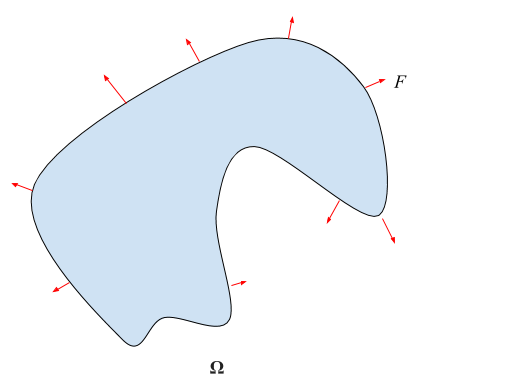
\includegraphics[width=0.7\linewidth]{img/eikonal_vision.png}
  \hfil \caption{распространение кривой со скоростью $F$}
  \label{fig:eikvis}

\end{figure}
\end{frame}
\stamp

\begin{frame}
\frametitle{Постановка задачи \\ Уравнение эйконала}
\begin{figure}[ht]
  \begin{equation}
    \label{eq:eikonal}
    \begin{cases}
      \begin{array}{ll}
        F(x) \| \nabla T(x) \| = 1, x \in \Omega \\
        T(x) = 0, x \in \Gamma
      \end{array}
    \end{cases}
  \end{equation}


\end{figure}


\begin{itemize}
\item $\Omega$ -- это область в $\mathbb{R}^2$;
\item $\Gamma$ -- начальное состояние кривой;
\item $\nabla$ -- градиент;
\item $\| \cdot \|$ -- евклидова норма.
\end{itemize}

\begin{figure}[ht]

\begin{equation}
  \label{eq:hje}
  \begin{cases}
    \begin{array}{ll}
      H(x, \nabla T(x)) = 0,\quad x \in \mathbb{R}^n  \\
      T(x) = 0, \quad  x \in \mathbb{R}^n,
    \end{array}
  \end{cases}
\end{equation}

Если $H(x,p) = |p| H(x,p/|p|) = |p| F(x)$, тогда мы получаем
обыкновенное уравнение эйконала для изотропного случая
\eqref{eq:eikonal}.

\end{figure}
\end{frame}
\stamp

% \begin{frame}
% \frametitle{Постановка задачи \\ Вязкостные решения}
% \begin{figure}[ht]
%   \begin{equation}
%   \label{eq:hje}
%   \begin{cases}
%     \begin{array}{ll}
%       H(x, \nabla T(x)) = 0,\quad x \in \mathbb{R}^n  \\
%       T(x) = 0, \quad  x \in \mathbb{R}^n,
%     \end{array}
%   \end{cases}
% \end{equation}

% где гамильтониан $H = H(x,\nabla T(x))$ непрерывная вещественная функция на
% $\mathbb{R}^n \times \mathbb{R}^n$ и $T(x) = 0$ -- начальные условия.

% Если $H(x,p) = |p| H(x,p/|p|) = |p| F(x)$, тогда мы получаем
% обыкновенное уравнение эйконала для изотропного случая
% \eqref{eq:eikonal}. Если гамильтониан имеет вид
% $H(x,p) = \|p\| F(x, \frac{p}{\|p\|})$, тогда мы имеем анизотропное
% уравнение эйконала.
% \end{figure}
% \end{frame}


\section{Методы решения}

\begin{frame}
  \frametitle{Численные методы решения\\Общая идея методов}
  \begin{itemize}
    \item Введем $\Delta x$ - шаг дискретизации, $i = -n, \cdots, n$
  \item Разобьем ось $x$ на набор точек сетки
    $x_i=i\Delta x$
  \item положим $T_{i} = T(i \Delta x)$ и
    $F_{i} = F(i \Delta x)$.

  \end{itemize}
  Введем также обозначение для разностных производных первого порядка:

  \begin{eqnarray}
    D^{+x}_iT(x_i) &=& \frac{T_{i+1} - T_{i}}{\Delta x} \\
    D^{-x}_iT(x_i) &=& \frac{T_{i} - T_{i-1}}{\Delta x}
  \end{eqnarray}

\end{frame}
\stamp
\begin{frame}
  \frametitle{Численные методы решения\\Общая идея методов}

\begin{figure}[H]
  \centering
  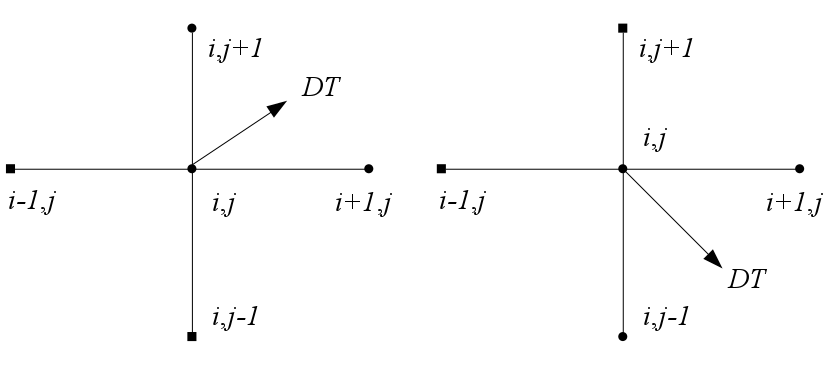
\includegraphics[width=0.8\linewidth]{img/upwind-schema.png}
  \hfil \caption{Пример разных направлений распространения}
  \label{fig:upwind-schema}

\end{figure}

  \begin{equation}
  \label{eq:godunov-schema}
  % \begin{cases}
  %   \begin{matrix}
       \max (D^{-x}_{ij}T, -D^{x}_{ij},0)^2 + \max (D^{-y}_{ij}T, -D^{y}_{ij},0)^2
  %   \end{matrix}
  % \end{cases}
  = \frac{1}{F_{ij}^2}
\end{equation}
\end{frame}
\stamp

\begin{frame}
\frametitle{Численные методы решения \\ Fast marching method на
    регулярной сетке}
\begin{figure}[ht]
  \centering
  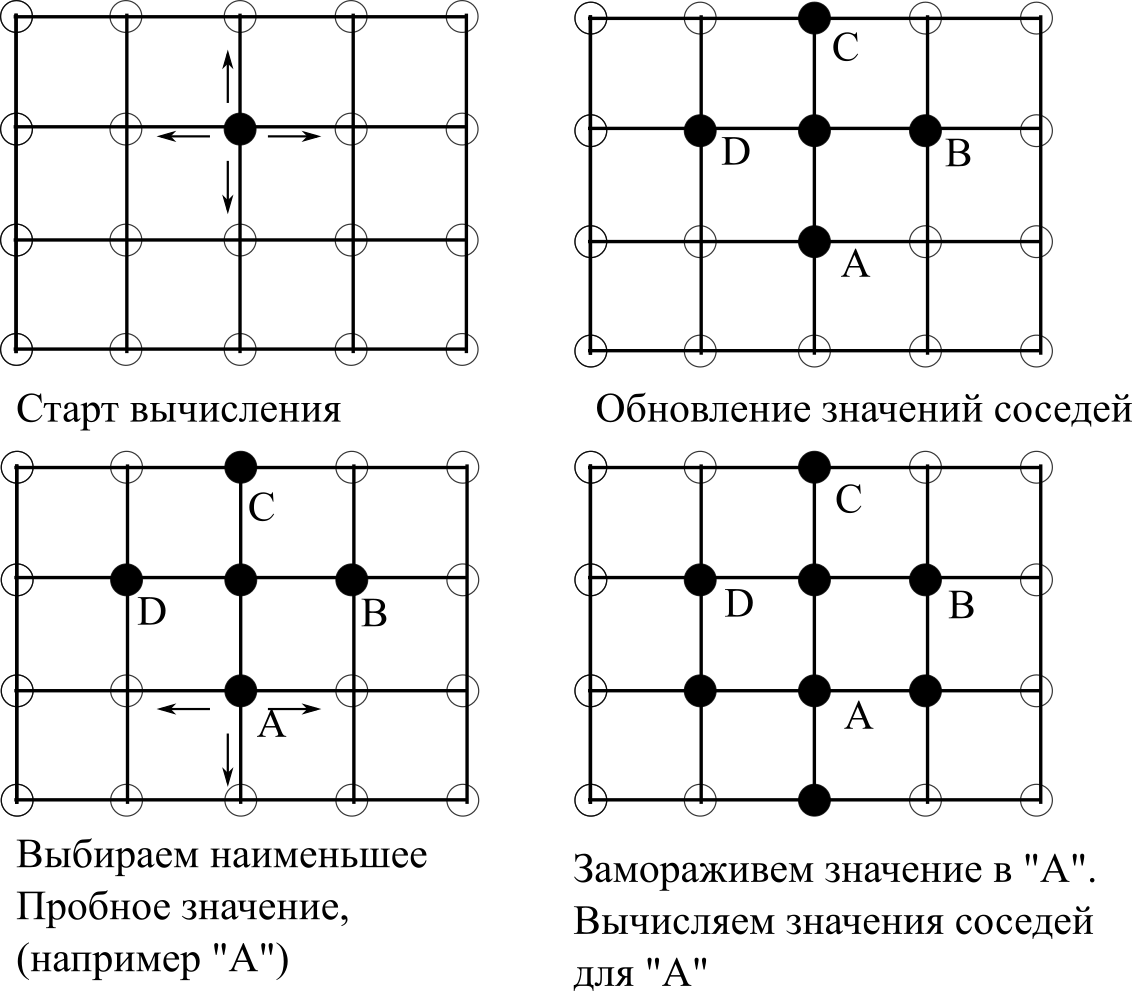
\includegraphics[width=0.7\linewidth]{img/fmm_expand.png}
  % \hfil \caption{\small{процедура обновления FMM}}
  \label{fig:eikvis}

\end{figure}
\end{frame}
\stamp


\begin{frame}
\frametitle{Численные методы решения \\ Fast marching method на регулярной сетке}
\begin{figure}[ht]
  \centering
  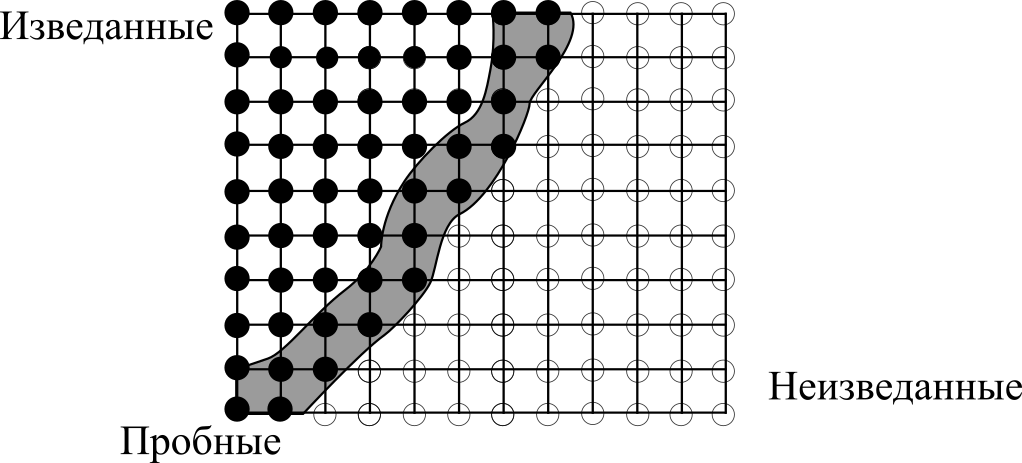
\includegraphics[width=\linewidth]{img/fmm_explain.png}
  \hfil \caption{ход работы FMM}
  \label{fig:eikvis}

\end{figure}
\end{frame}
\stamp

\begin{frame}
  \frametitle{Численные методы решения \\ Fast marching method на
    регулярной сетке}
  \begin{figure}[ht]
  \centering
  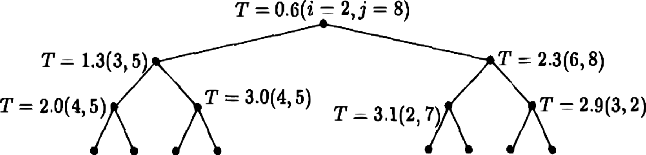
\includegraphics[width=0.9\linewidth]{img/minheap.png}
  \hfil \caption{Пример пираммиды для $T$}
  \label{fig:eikvis}
\end{figure}
\begin{itemize}
  \item Вычисление значения в узле: $O(1)$;
  \item Выбрать наименьшую вершину: $O(1)$;
  \item Вставка новой вершины: $O(\log n)$;
  \item Число итераций не более чем $n$, где $n$ -- число узлов
  \end{itemize}

  сложность FMM
  ограничивается сверху $O(n \log n)$
  
\end{frame}
\stamp

\begin{frame}
  \frametitle{Численные методы решения \\ Fast sweeping method на
    регулярной сетке}
  \begin{figure}[ht]
  \centering
  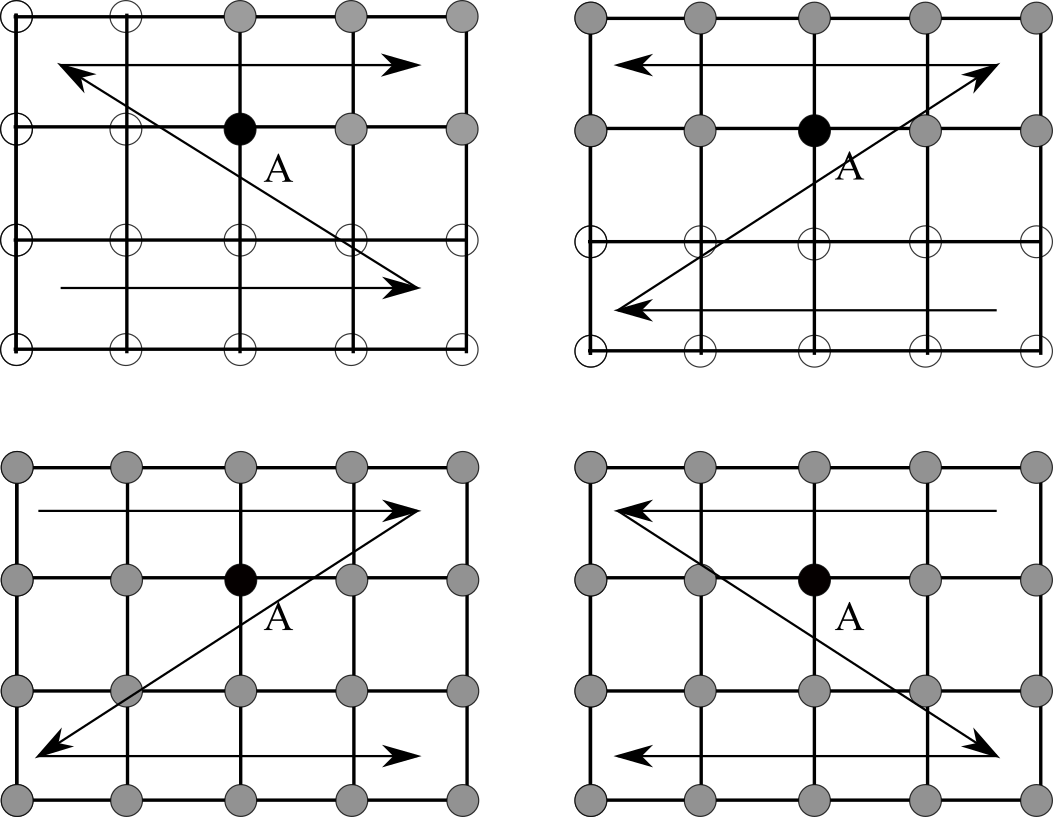
\includegraphics[width=0.7\linewidth]{img/fsm_expand.png}
  \hfil \caption{процедура выметания FSM}
  \label{fig:eikvis}

\end{figure}
\end{frame}
\stamp

\begin{frame}
  \frametitle{Численные методы решения \\ Fast sweeping method на
    регулярной сетке}

  \begin{itemize}
  \item Вычисление значения в узле: $O(1)$;
  \item при наличии $n$ вершин, получаем сложность $O(n)$
  \end{itemize}
  \vspace{1em}
  Однако скорость работы будет сильно зависеть от функции $F(x)$:
  \begin{itemize}
  \item В случае простого устройства $F(x)$ необходимо 4 итерации
  \item Если устройство сложное, заранее неизвестно число итераций
  \end{itemize}
  
  
  
\end{frame}
\stamp


\begin{frame}


  \frametitle{Численные методы решения \\Fast sweeping method на нерегулярной сетке}
  
\begin{figure}[H]
  \centering
  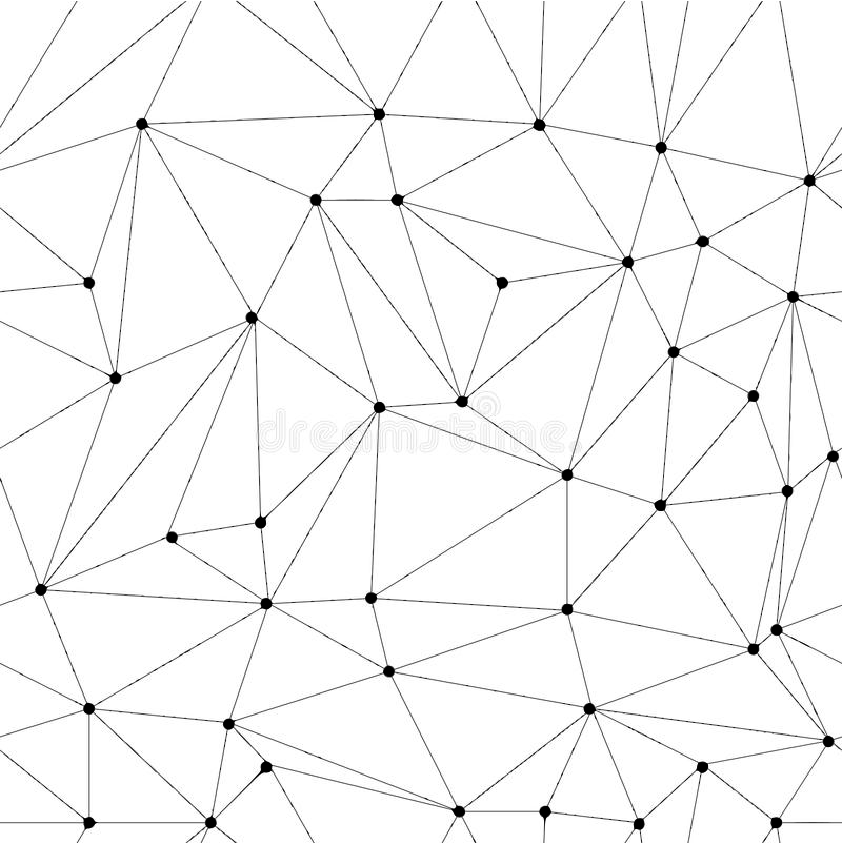
\includegraphics[width=0.5\linewidth]{img/triangle-mesh.png}
  \hfil \caption{Пример треугольной сетки}
  \label{fig:triangle-front}

\end{figure}

  
\end{frame}
\stamp


\begin{frame}
  \frametitle{Численные методы решения \\Fast sweeping method на нерегулярной сетке}
  
\begin{figure}[H]
  \centering
  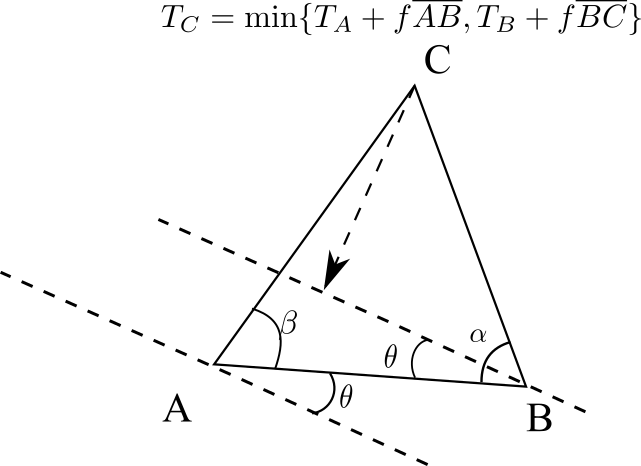
\includegraphics[width=0.7\linewidth]{img/triangle-front-slide.png}
  \hfil \caption{Изменение значения в вершине С, на треугольной сетке}
  \label{fig:triangle-front}

\end{figure}

  
\end{frame}
\stamp

\begin{frame}
  \frametitle{Численные методы решения \\Fast sweeping method на нерегулярной сетке}

\begin{enumerate}
\item если $|T_B-T_A| \le c f_C$, тогда
  \begin{equation*}
    \theta = arcsin \left(\frac{|T_B-T_A|}{c f_C}\right);
  \end{equation*}
  \begin{enumerate}
  \item если $\max (0,\alpha - \frac{\pi}{2}) \le \theta \le
    \frac{\pi}{2} - \beta$ или $\alpha - \frac{\pi}{2} \le \theta \le
    \min(0, \frac{\pi}{2} - \beta)$, тогда
    \begin{equation*}
      \begin{aligned}{c}
        h = \overline{CP} = a \sin(\alpha - \theta); H =
        \overline{CQ}=
        b \sin (\beta + \theta);\\
        T_C = \min\{T_C,0.5(h f_C + T_B)+0.5(H f_C + T_A)\};
      \end{aligned}
    \end{equation*}
  \item иначе
    \begin{equation*}
      T_C = \min\{T_C,T_A+b f_C, T_B + a f_C\};
    \end{equation*}
  \end{enumerate}
\item иначе
  \begin{equation*}
    T_C = \min\{T_C,T_A+b f_C, T_B + a f_C\};
  \end{equation*}

\end{enumerate}
\end{frame}
\stamp


\begin{frame}
  \frametitle{Численные методы решения \\Fast sweeping method на нерегулярной сетке}
  
\begin{figure}[H]
  \centering
  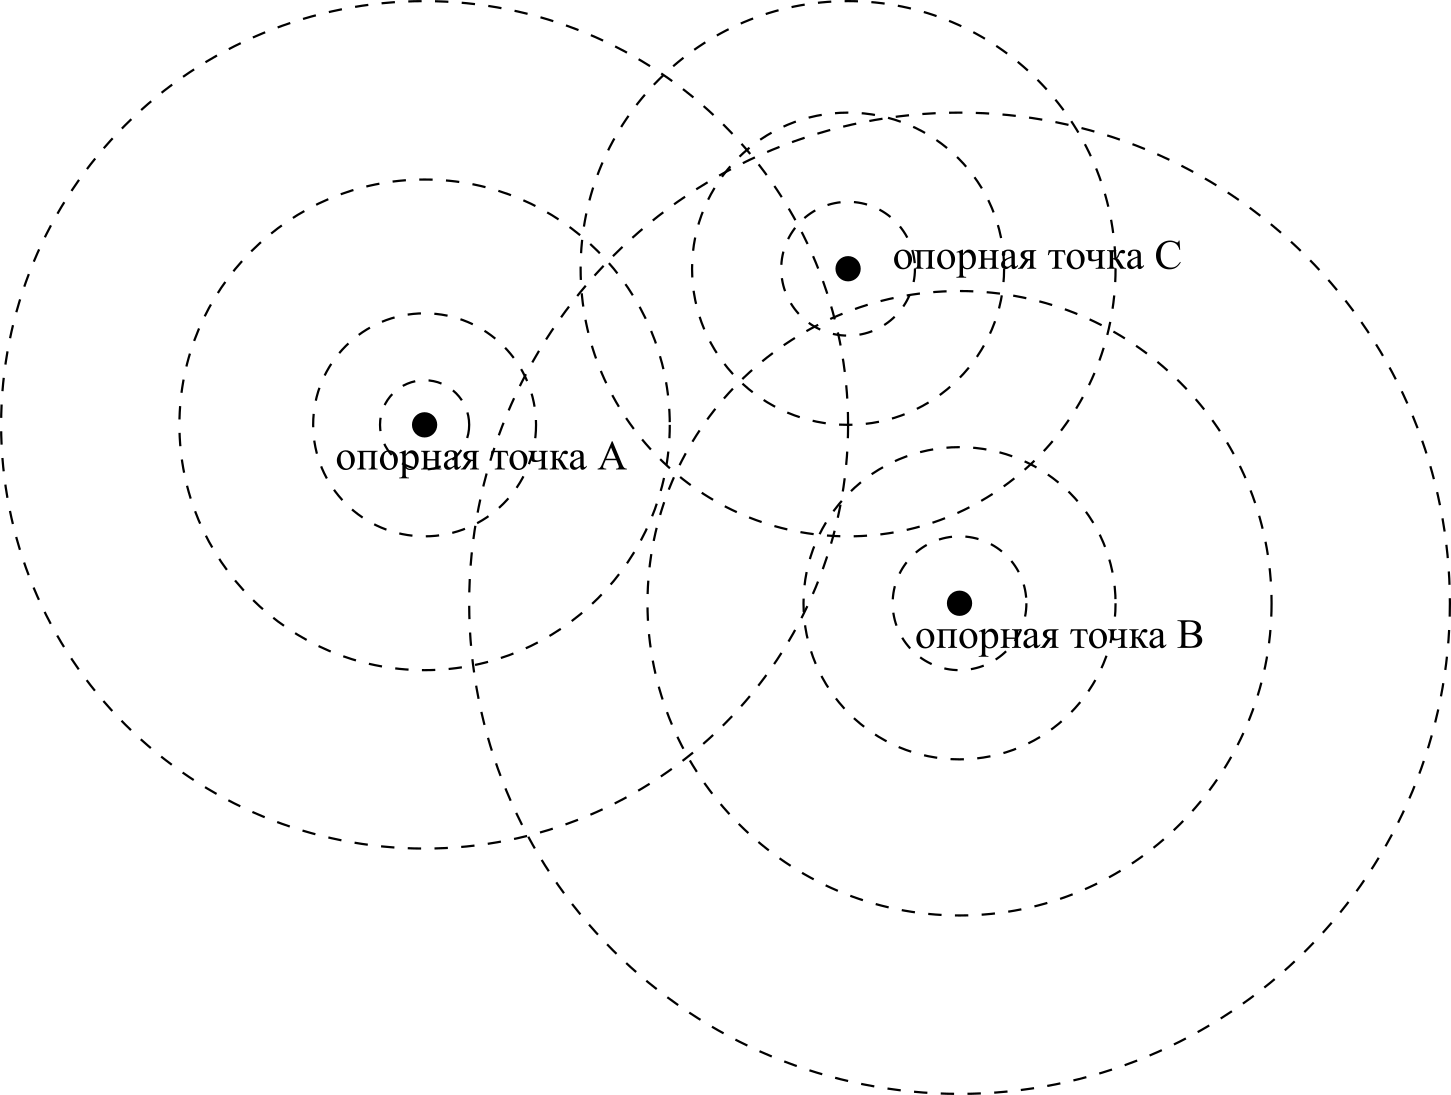
\includegraphics[width=0.7\linewidth]{img/refpoints.png}
  \hfil \caption{Опорные точки}
  \label{fig:triangle-front}

\end{figure}

  
\end{frame}
\stamp


\begin{frame}
  \frametitle{Численные методы решения \\
Fast sweeping method для анизотропного случая}


\begin{equation}
  \label{eq:hje}
  \begin{cases}
    \begin{array}{ll}
      H(x, \nabla T(x)) = 0,\quad x \in \mathbb{R}^n  \\
      T(x) = 0, \quad  x \in \mathbb{R}^n,
    \end{array}
  \end{cases}
\end{equation}

Если гамильтониан имеет вид $H(x,p) = \|p\| F(x, \frac{p}{\|p\|})$,
тогда мы получим анизотропное уравнение эйконала.


\begin{figure}[H]
  \centering
  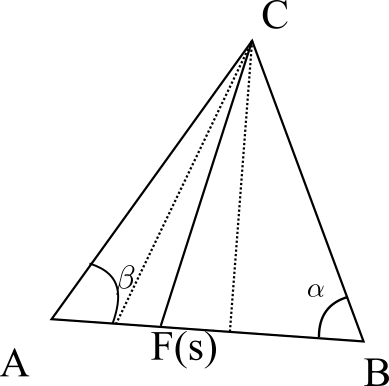
\includegraphics[width=0.3\linewidth]{img/anisotropy.png}
  \hfil \caption{Локальное решение в анизотропном случае}
  \label{fig:triangle-front}

\end{figure}


\end{frame}
\stamp


\begin{frame}
  \frametitle{Численные методы решения \\
Fast sweeping method для анизотропного случая}

\begin{equation}
  \label{eq:2}
  T_C(s) = sT_B + (1-s)T_A + \frac{d(s)}{v_g(C)} \rightarrow \min,
\end{equation}

где $d(s) = \overline{CF(s)} = \sqrt{b^2+c^2s^2-2bcs \cos \beta}$, а
параметр $v_g$ - так называемый вектор группы скоростей, который
указывает в направлении действия луча $CF(s)$

\begin{equation}
  \label{eq:3}
  v_g(x,p) = \left| \frac{dx}{dt} \right| = \left| \nabla_p H  \right|
\end{equation}


\end{frame}
\stamp

\section{Примеры}

\begin{frame}
  \frametitle{Примеры \\ Евклидово расстояние}

  \begin{equation}
    \label{eq:eik-sur}
    \begin{cases}
      \begin{array}{ll}
        \| \nabla T(x) \| = \frac{1}{F(x)}, x \in \Omega \\
        T(x) = 0, x \in \Gamma
      \end{array}\end{cases}
  \end{equation}


  \begin{figure}[ht]
    \begin{minipage}[h]{0.49\linewidth}
      \centering
      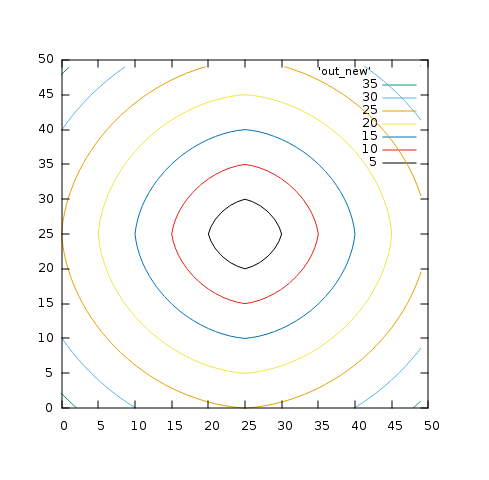
\includegraphics[width=0.7\linewidth]{img/eikonal_simple_surface.png}
      \hfil \caption{Линии уровня эйконала с $F\equiv 1$ }
      \label{fig:eikonal-surface}

    \end{minipage}
    \begin{minipage}[ht]{0.49\linewidth}
      % \centering
      \centering
      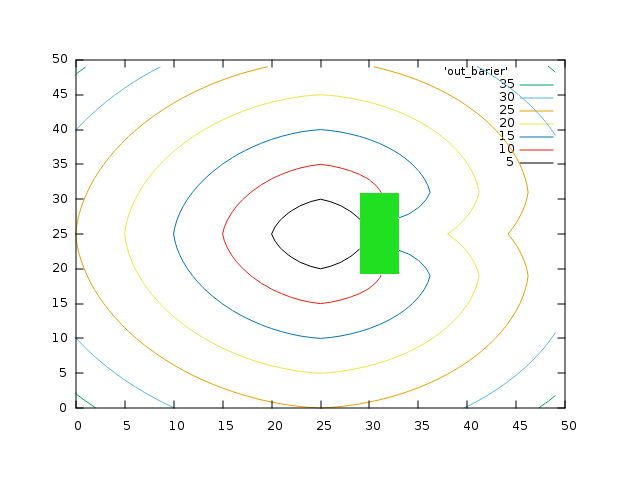
\includegraphics[width=0.7\linewidth]{img/barier_surface.png}
      \hfil \caption{Линии уровня эйконала с $F\equiv 1$, с препятствием}
      \label{fig:barier_surface}
    \end{minipage}
  \end{figure}

\end{frame}
\stamp

\begin{frame}
  \frametitle{Примеры \\ Множество достижимости импульсной системы}


\begin{equation}
  \label{system_s}
  \begin{array}{l}
    \dot{x}(t)=E \cdot F(x)v(t), \quad x(0)=x_0, \\[8pt]
    v(t)\geq 0  \qquad \forall\, t\in T = [0,t_1], \qquad
    \displaystyle\int_{0}^{t_1} ||v(t)||dt\leq V.
  \end{array} 
\end{equation}

Здесь
\begin{itemize}
  \item $E$ --- единичная матрица.
  \item $x(\cdot)$ --- абсолютно непрерывная вектор-функция
    (траектория), $x(t)\in {\mathbb R}^n,$
  \item $v(\cdot)$ --- измеримая существенно ограниченная
    вектор-функция (управление),
  
  \item $V$ --- заданная величина интегрального ресурса управления
    $v$.
\end{itemize}

\end{frame}
\stamp


\begin{frame}
  \frametitle{Примеры \\ Множество достижимости импульсной системы}

\begin{equation*}
  \begin{aligned}[b]
    &\dot{x_1}(t) = (1/((x_1(t)+0.1) * (x_2(t)+0.1))v_1(t), & x_1(0)=50\\
    &\dot{x_2}(t) = (1/((x_1(t)+0.1) * (x_2(t)+0.1))v_2(t), & x_2(0) = 50\\[8pt]
    &v_1(t) \ge 0, v_2(t) \ge 0 \\
    &\int_{0}^{1} \sqrt{(v_1(t)^2) + (v_2(t))^2} dt \le V
  \end{aligned}
\end{equation*}

  
\end{frame}
\stamp

\begin{frame}
  \frametitle{Примеры \\ Множество достижимости импульсной системы}

  \begin{figure}[ht]
    \begin{minipage}[h]{0.49\linewidth}
      \centering
      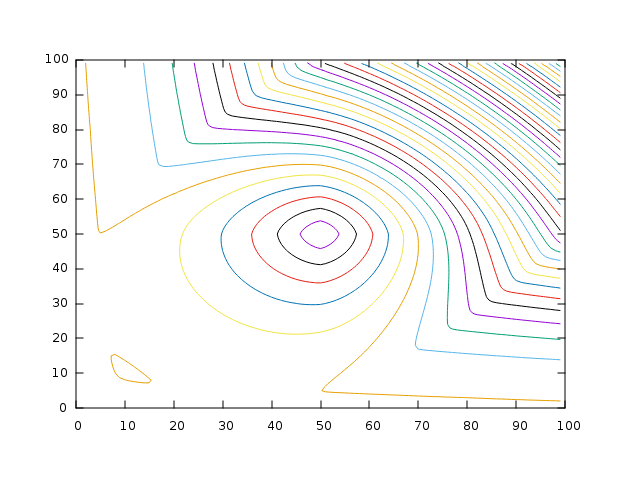
\includegraphics[width=0.9\linewidth]{img/impulse-example-levels.png}
      \hfil \caption{Линии уровня множества достижимости }
      \label{fig:eikonal-surface}

    \end{minipage}
    \begin{minipage}[ht]{0.49\linewidth}
      % \centering
      \centering
      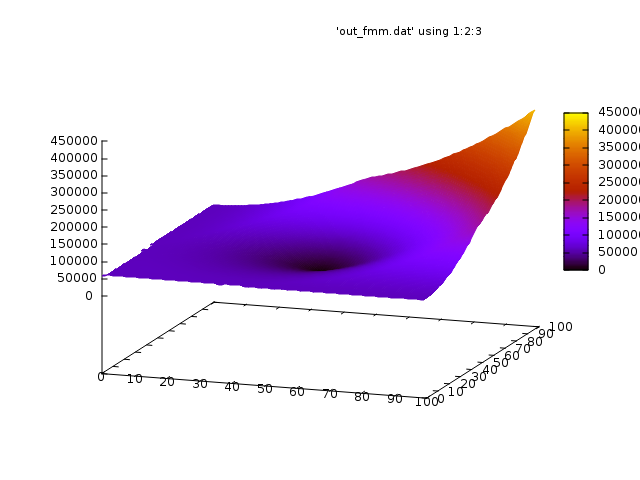
\includegraphics[width=0.9\linewidth]{img/impulse-example.png}
      \hfil \caption{трехмерный вид интегральной воронки}
      \label{fig:barier_surface}
    \end{minipage}
  \end{figure}

\end{frame}
\stamp

\begin{frame}
  \frametitle{Примеры \\ Shape from shading}

  \begin{figure}[ht]
    \begin{minipage}[h]{0.49\linewidth}
      \begin{equation}
        \label{eq:sfs:1}
        E_i=\mu L_s,
      \end{equation}

      \begin{equation}
        \label{eq:sfs:4}
        L_s=\frac{\alpha}{\pi}E_s,
      \end{equation}

      \begin{equation}
        \label{eq:sfs:5}
        E_s = I_0\frac{cos(\theta_i)}{r^2},
      \end{equation}
      Из \eqref{eq:sfs:1}, \eqref{eq:sfs:4} и \eqref{eq:sfs:5} получим
      яркость
      изображения:
      
      \begin{equation}
        \label{eq:sfs:6}
        E_i = \sigma\frac{cos(\theta_i)}{r^2},
      \end{equation}

    \end{minipage}
    \begin{minipage}[ht]{0.49\linewidth}
      % \centering
      \centering
      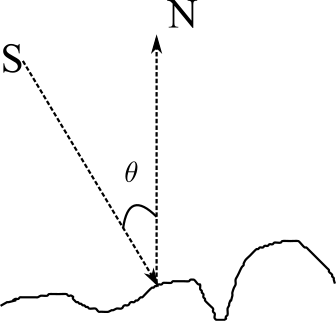
\includegraphics[width=0.9\linewidth]{img/sfs-explain.png}
      \hfil \caption{Пример поверхности с источником света $S$ и
        нормалью $N$}
      \label{fig:barier_surface}
    \end{minipage}
  \end{figure}

\end{frame}
\stamp

\begin{frame}
  \frametitle{Примеры \\ Shape from shading}

  \begin{figure}[ht]
    \begin{minipage}[h]{0.49\linewidth}
      \centering
      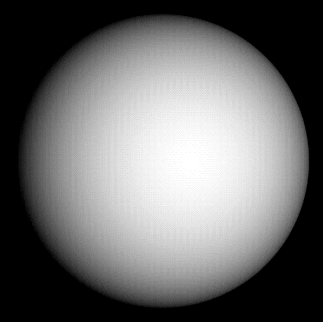
\includegraphics[width=0.9\linewidth]{img/sphere_in.png}
      \hfil \caption{Сфера исходное изображение}
      \label{fig:ex:1:in}

    \end{minipage}
    \begin{minipage}[ht]{0.49\linewidth}
      \centering
      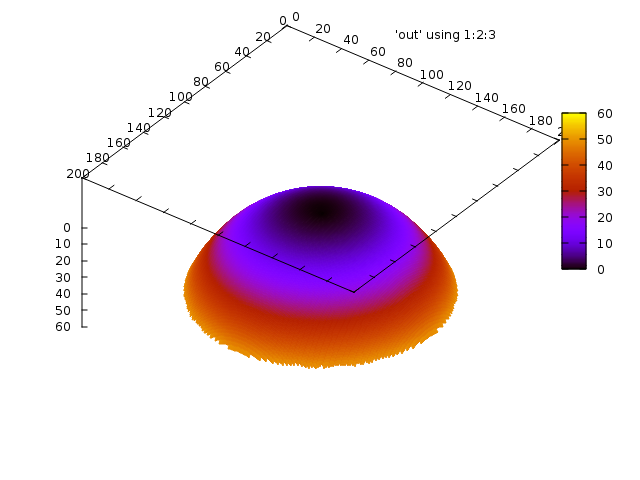
\includegraphics[width=0.9\linewidth]{img/sphere.png}
      \hfil \caption{Трехмерная поверхность сферы по фотографии}
      \label{fig:ex:1:out}

    \end{minipage}
  \end{figure}

\end{frame}
\stamp

\begin{frame}
  \frametitle{Примеры \\ Shape from shading}

  \begin{figure}[ht]
    \begin{minipage}[h]{0.49\linewidth}
      \centering
      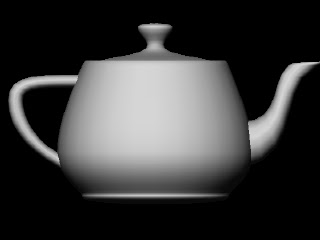
\includegraphics[width=0.9\linewidth]{img/teapot_in.jpg}
      \hfil \caption{Чайник исходное изображение}
      \label{fig:ex:1:in}

    \end{minipage}
    \begin{minipage}[ht]{0.49\linewidth}
      \centering
      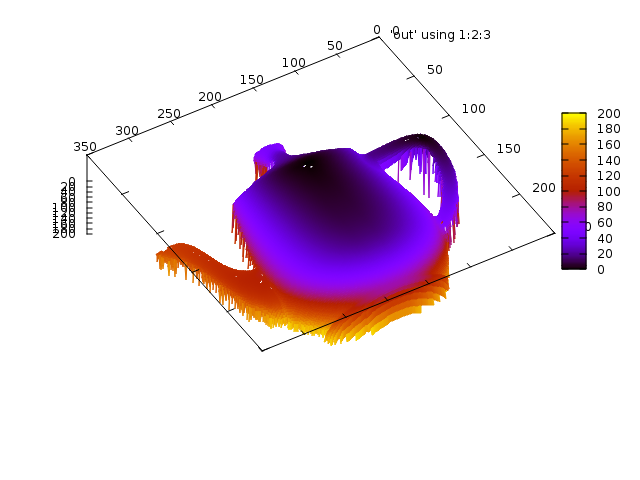
\includegraphics[width=0.9\linewidth]{img/teapot.png}
      \hfil \caption{Трехмерная поверхность чайника по фотографии}
      \label{fig:ex:1:out}

    \end{minipage}
  \end{figure}

\end{frame}
\stamp


\begin{frame}
  \frametitle{Примеры \\ Shape from shading}

  \begin{figure}[ht]
    \begin{minipage}[h]{0.49\linewidth}
      \centering
      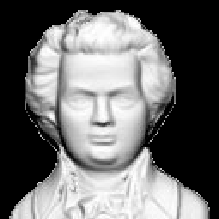
\includegraphics[width=0.9\linewidth]{img/mozart_in.png}
      \hfil \caption{Моцарт исходное изображение}
      \label{fig:ex:1:in}

    \end{minipage}
    \begin{minipage}[ht]{0.49\linewidth}
      \centering
      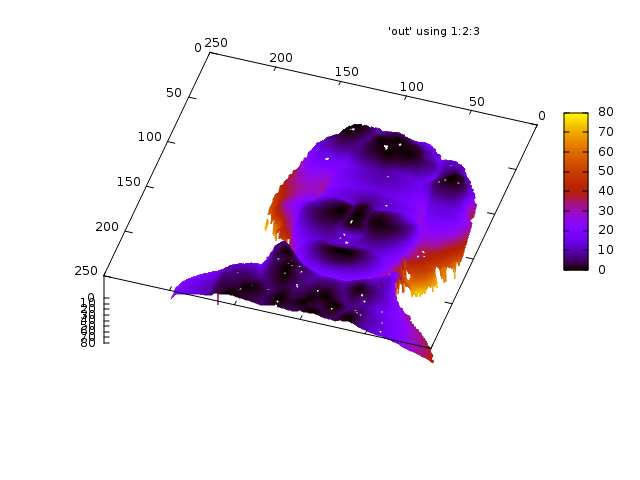
\includegraphics[width=0.9\linewidth]{img/mozart.png}
      \hfil \caption{Трехмерная поверхность моцарта по фотографии}
      \label{fig:ex:1:out}

    \end{minipage}
  \end{figure}

\end{frame}
\stamp

\begin{frame}
  \frametitle{Примеры \\ Shape from shading}

  \begin{figure}[ht]
    \begin{minipage}[h]{0.49\linewidth}
      \centering
      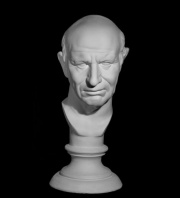
\includegraphics[width=0.9\linewidth]{img/man_in.jpg}
      \hfil \caption{исходная фотография}
      \label{fig:ex:4:in}

    \end{minipage}
    \begin{minipage}[ht]{0.49\linewidth}
      \centering
      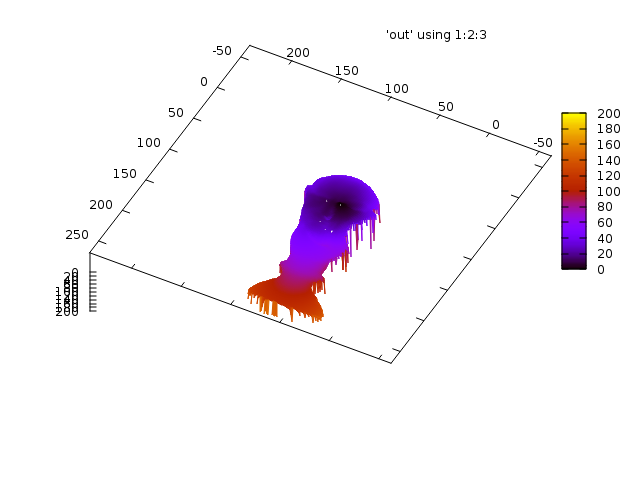
\includegraphics[width=0.9\linewidth]{img/man_all.png}
      \hfil \caption{Трехмерная поверхность по фотографии общая}
      \label{fig:ex:4:out1}
    \end{minipage}
  \end{figure}

\end{frame}
\stamp

\begin{frame}
  \frametitle{Заключение}
  \begin{itemize}
  \item Разработаны реализации алгоритмов численных решений уравнений
    эйконала на языке C;
  \item Проведены численные эксперименты с параллельным вариантом FSM
  \item методы применены к задаче восстановления формы тела по черно-белому
    снимку, однако высокая точность достигается только для
    синтезированных изображений;
  \item Применение к задаче аппроксимации множества достижимости
    импульсной системы в качестве помощника в поиске аналитического
    решения и генератора иллюстраций
  \end{itemize}

\end{frame}
\stamp


\begin{frame}
  \Huge Спасибо за внимание
\end{frame}
\stamp


\end{document}

%%% Local Variables:
%%% mode: latex
%%% TeX-master: t
%%% End:
